\documentclass[a4paper, 14pt]{extarticle}%тип документа

%Русский язык
\usepackage[T2A]{fontenc} %кодировка
\usepackage[utf8]{inputenc} %кодировка исходного кода
\usepackage[english,russian]{babel} %локализация и переносы

%отступы 
\usepackage[left=2cm,right=2cm,top=2cm,bottom=3cm,bindingoffset=0cm]{geometry}

%Вставка картинок
\usepackage{graphicx}
\usepackage{wrapfig, caption}
\graphicspath{}
\DeclareGraphicsExtensions{.pdf,.png,.jpg, .jpeg}
\newcommand\ECaption[1]{%
     \captionsetup{font=footnotesize}%
     \caption{#1}}

%Таблицы
\usepackage[table,xcdraw]{xcolor}
\usepackage{booktabs}

%Графики
\usepackage{pgfplots}
\pgfplotsset{compat=1.9}

%Математика
\usepackage{amsmath, amsfonts, amssymb, amsthm, mathtools}

%Заголовок
\author{Подлесный Артём \\ группа 827}
\title{Работа 2.1 \\ Опыты Франка-Герца.}

\begin{document}
\maketitle

\section*{Краткая теория}

С помощью опыта Франка-Герца можно подтвердить дискретность уровней энергии атома Гелия, а так же измерить энергию первого уровня. Схема опыта представлена на рис.1.

\begin{figure}[h]
\begin{center}
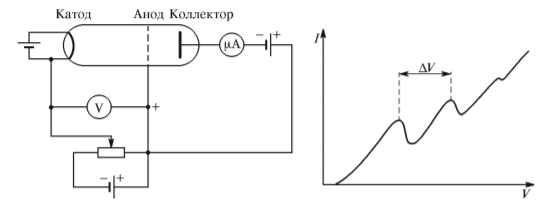
\includegraphics[width=0.9\textwidth]{teor1}
\ECaption{a) Схема опыта Франка-Герца. \\ б) Схематическая зависимость тока коллектора и напряжения на аноде.}
\end{center}
\end{figure}

Такой график показывает дискретность уровней энергии: если энергия электронов недостаточна, чтобы при столкновении перревести атом в возбужденное состояние, то соударения с атомами упругие -- электроны не теряют энергии, поэтому способны долететь до коллектора. Когда энергия превышает первый уровень, то соударения с атомами неупругие, так как электрон передает энергию атому, поэтому ток резко уменьшается. Аналогично происходит для второго пика: если энергия электронов достаточна, чтобы дважды возбудить атом гелия, то происходит повторное столкновение с атомом тоже неупругое. 

Так как электрон при соударении передает энергию, равную энергии первого уровня, то $\Delta V$ между двумя пиками будет равна этой энергии. Так как в схеме присутствует контактная разность напряжений между анодом и катодом, то первый пик не соответсвует $\Delta V$.

Зависимость $I_k(V_a)$ может измеряться динамическим, или статическим методом.

\section*{Динамический метод}

В этом методе ускоряющее напряжение $V_a$ подается с понижающего трансформатора на анод, а ток с коллектора подается на экран осциллографа. При переключении развертки на X-Y можно наблюдать искомую зависимость. Для разных значений задерживающего напряжения она представлена на рис.2.
\begin{figure}[h]
\begin{minipage}[h]{0.32\linewidth}
\center{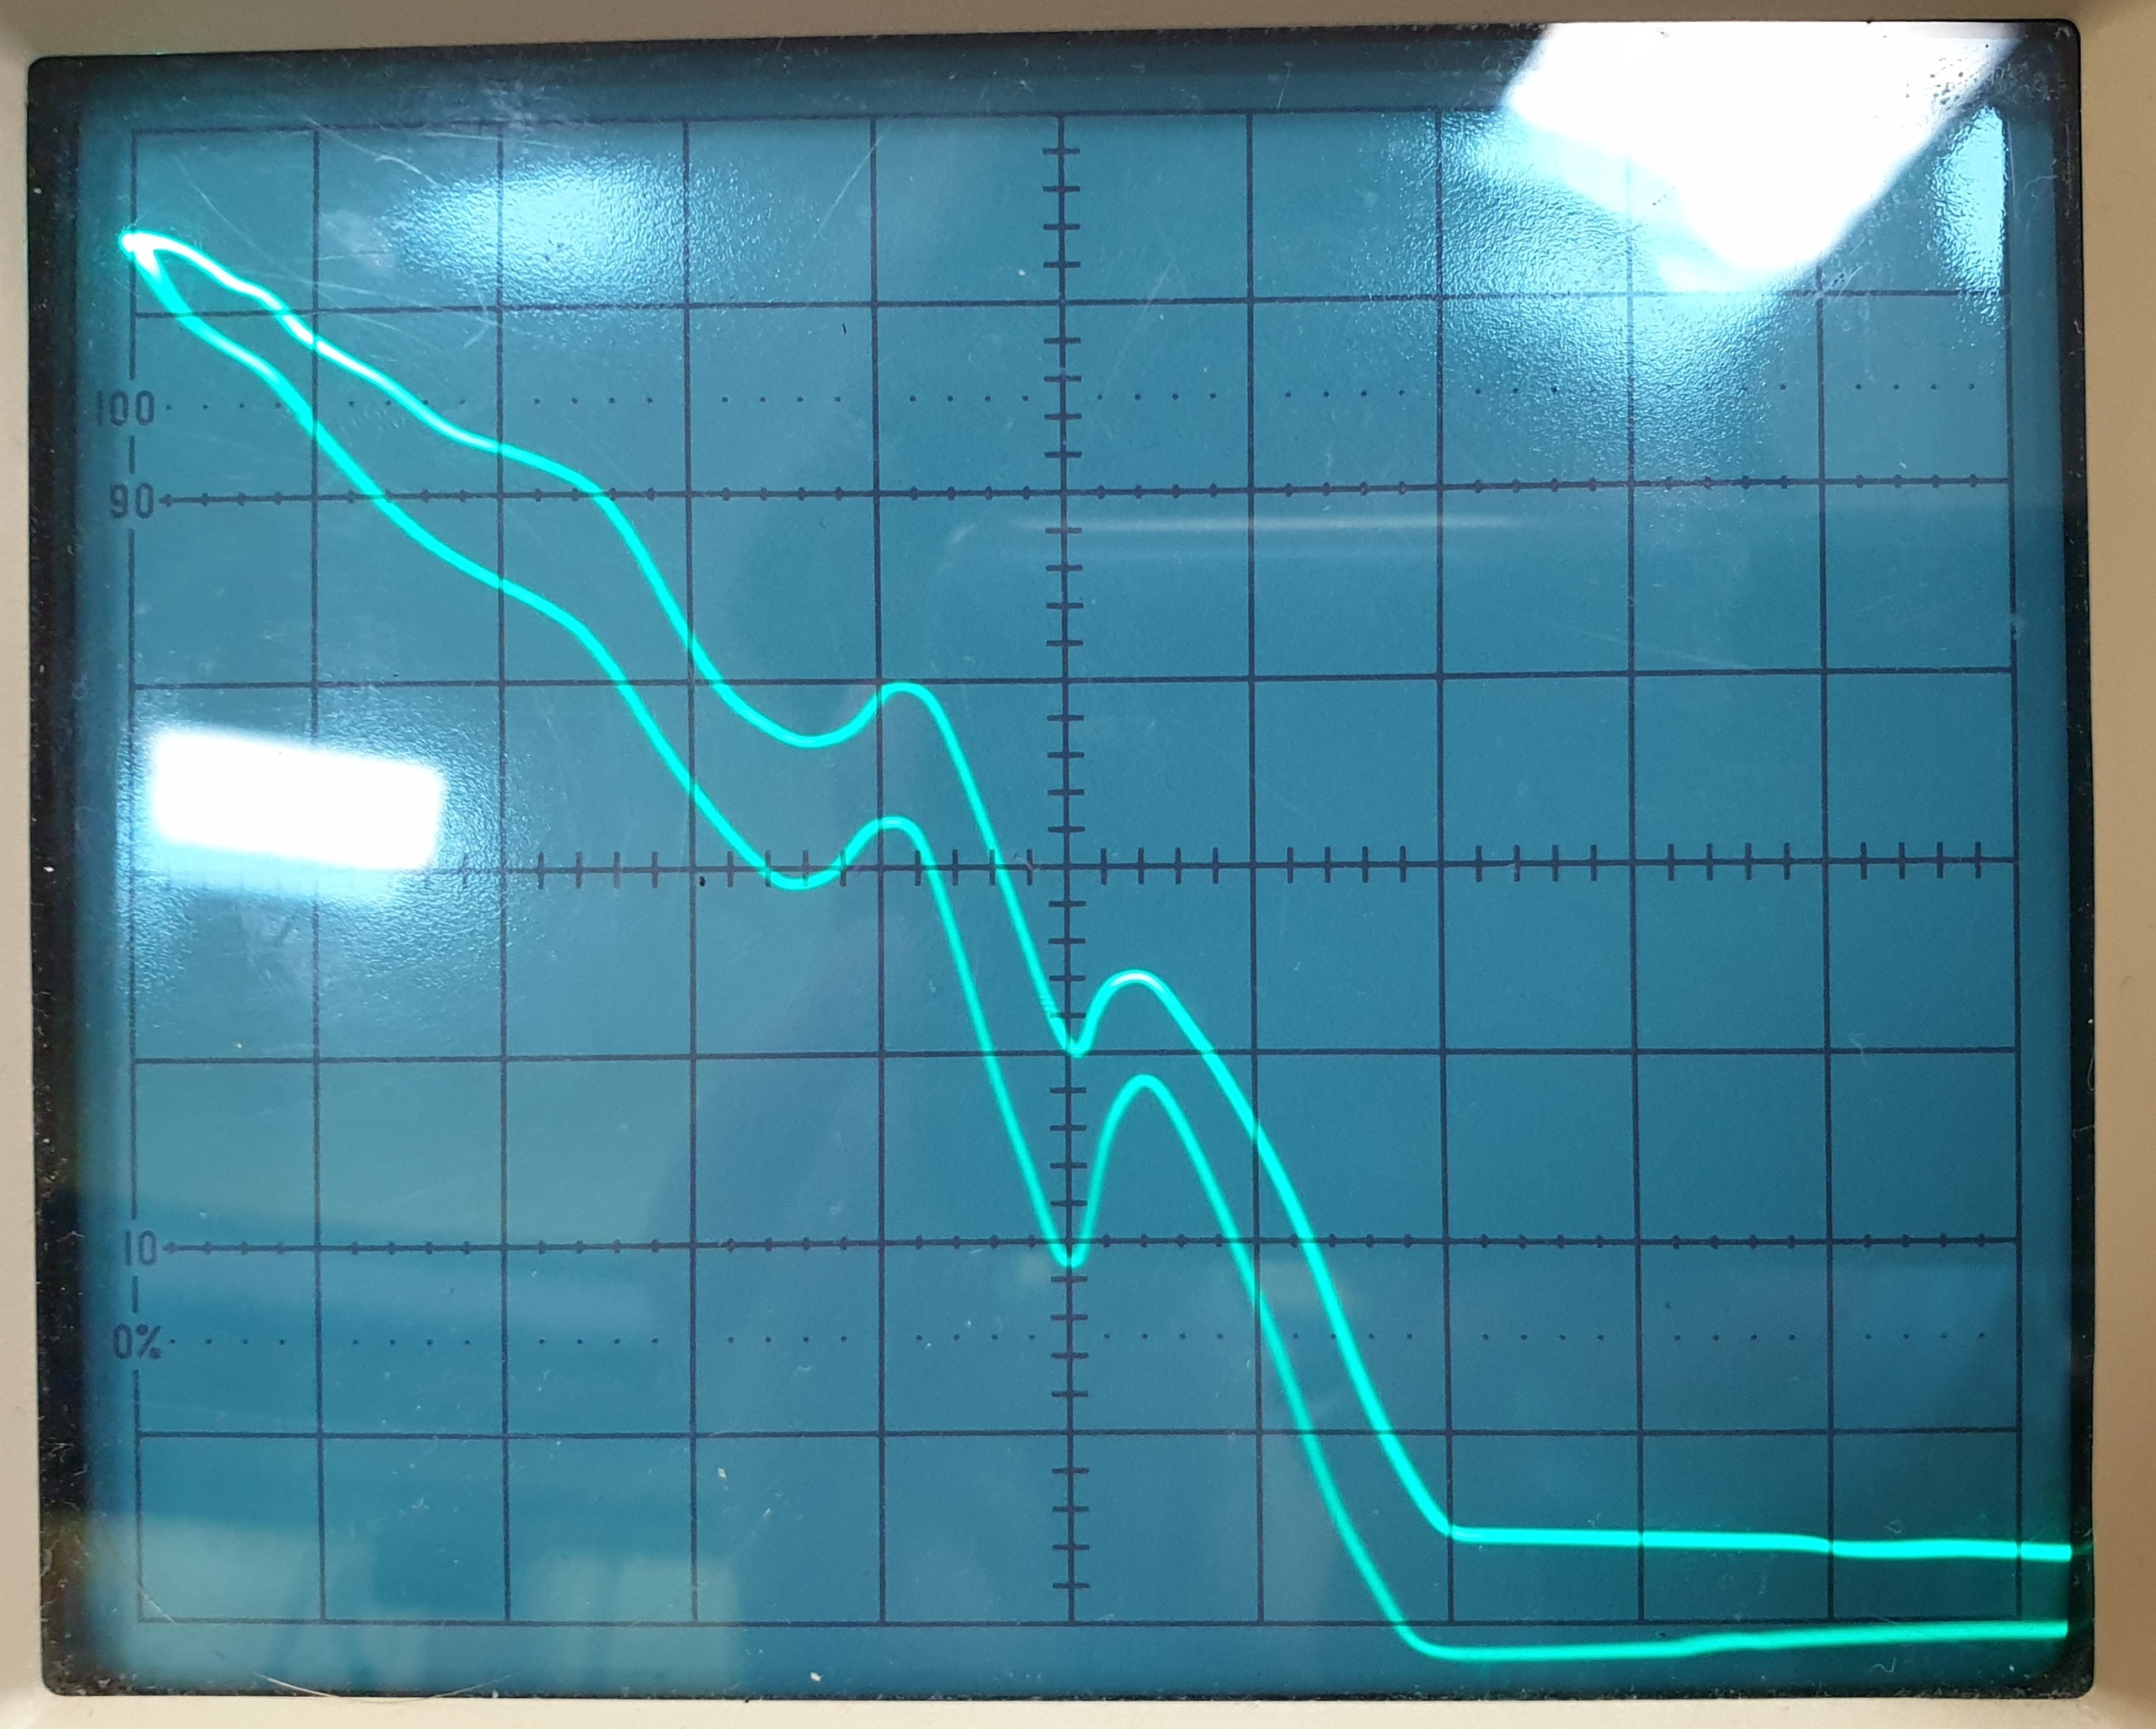
\includegraphics[width=1\linewidth]{din4V} \\ (4B)}
\end{minipage}
\hfill
\begin{minipage}[h]{0.32\linewidth}
\center{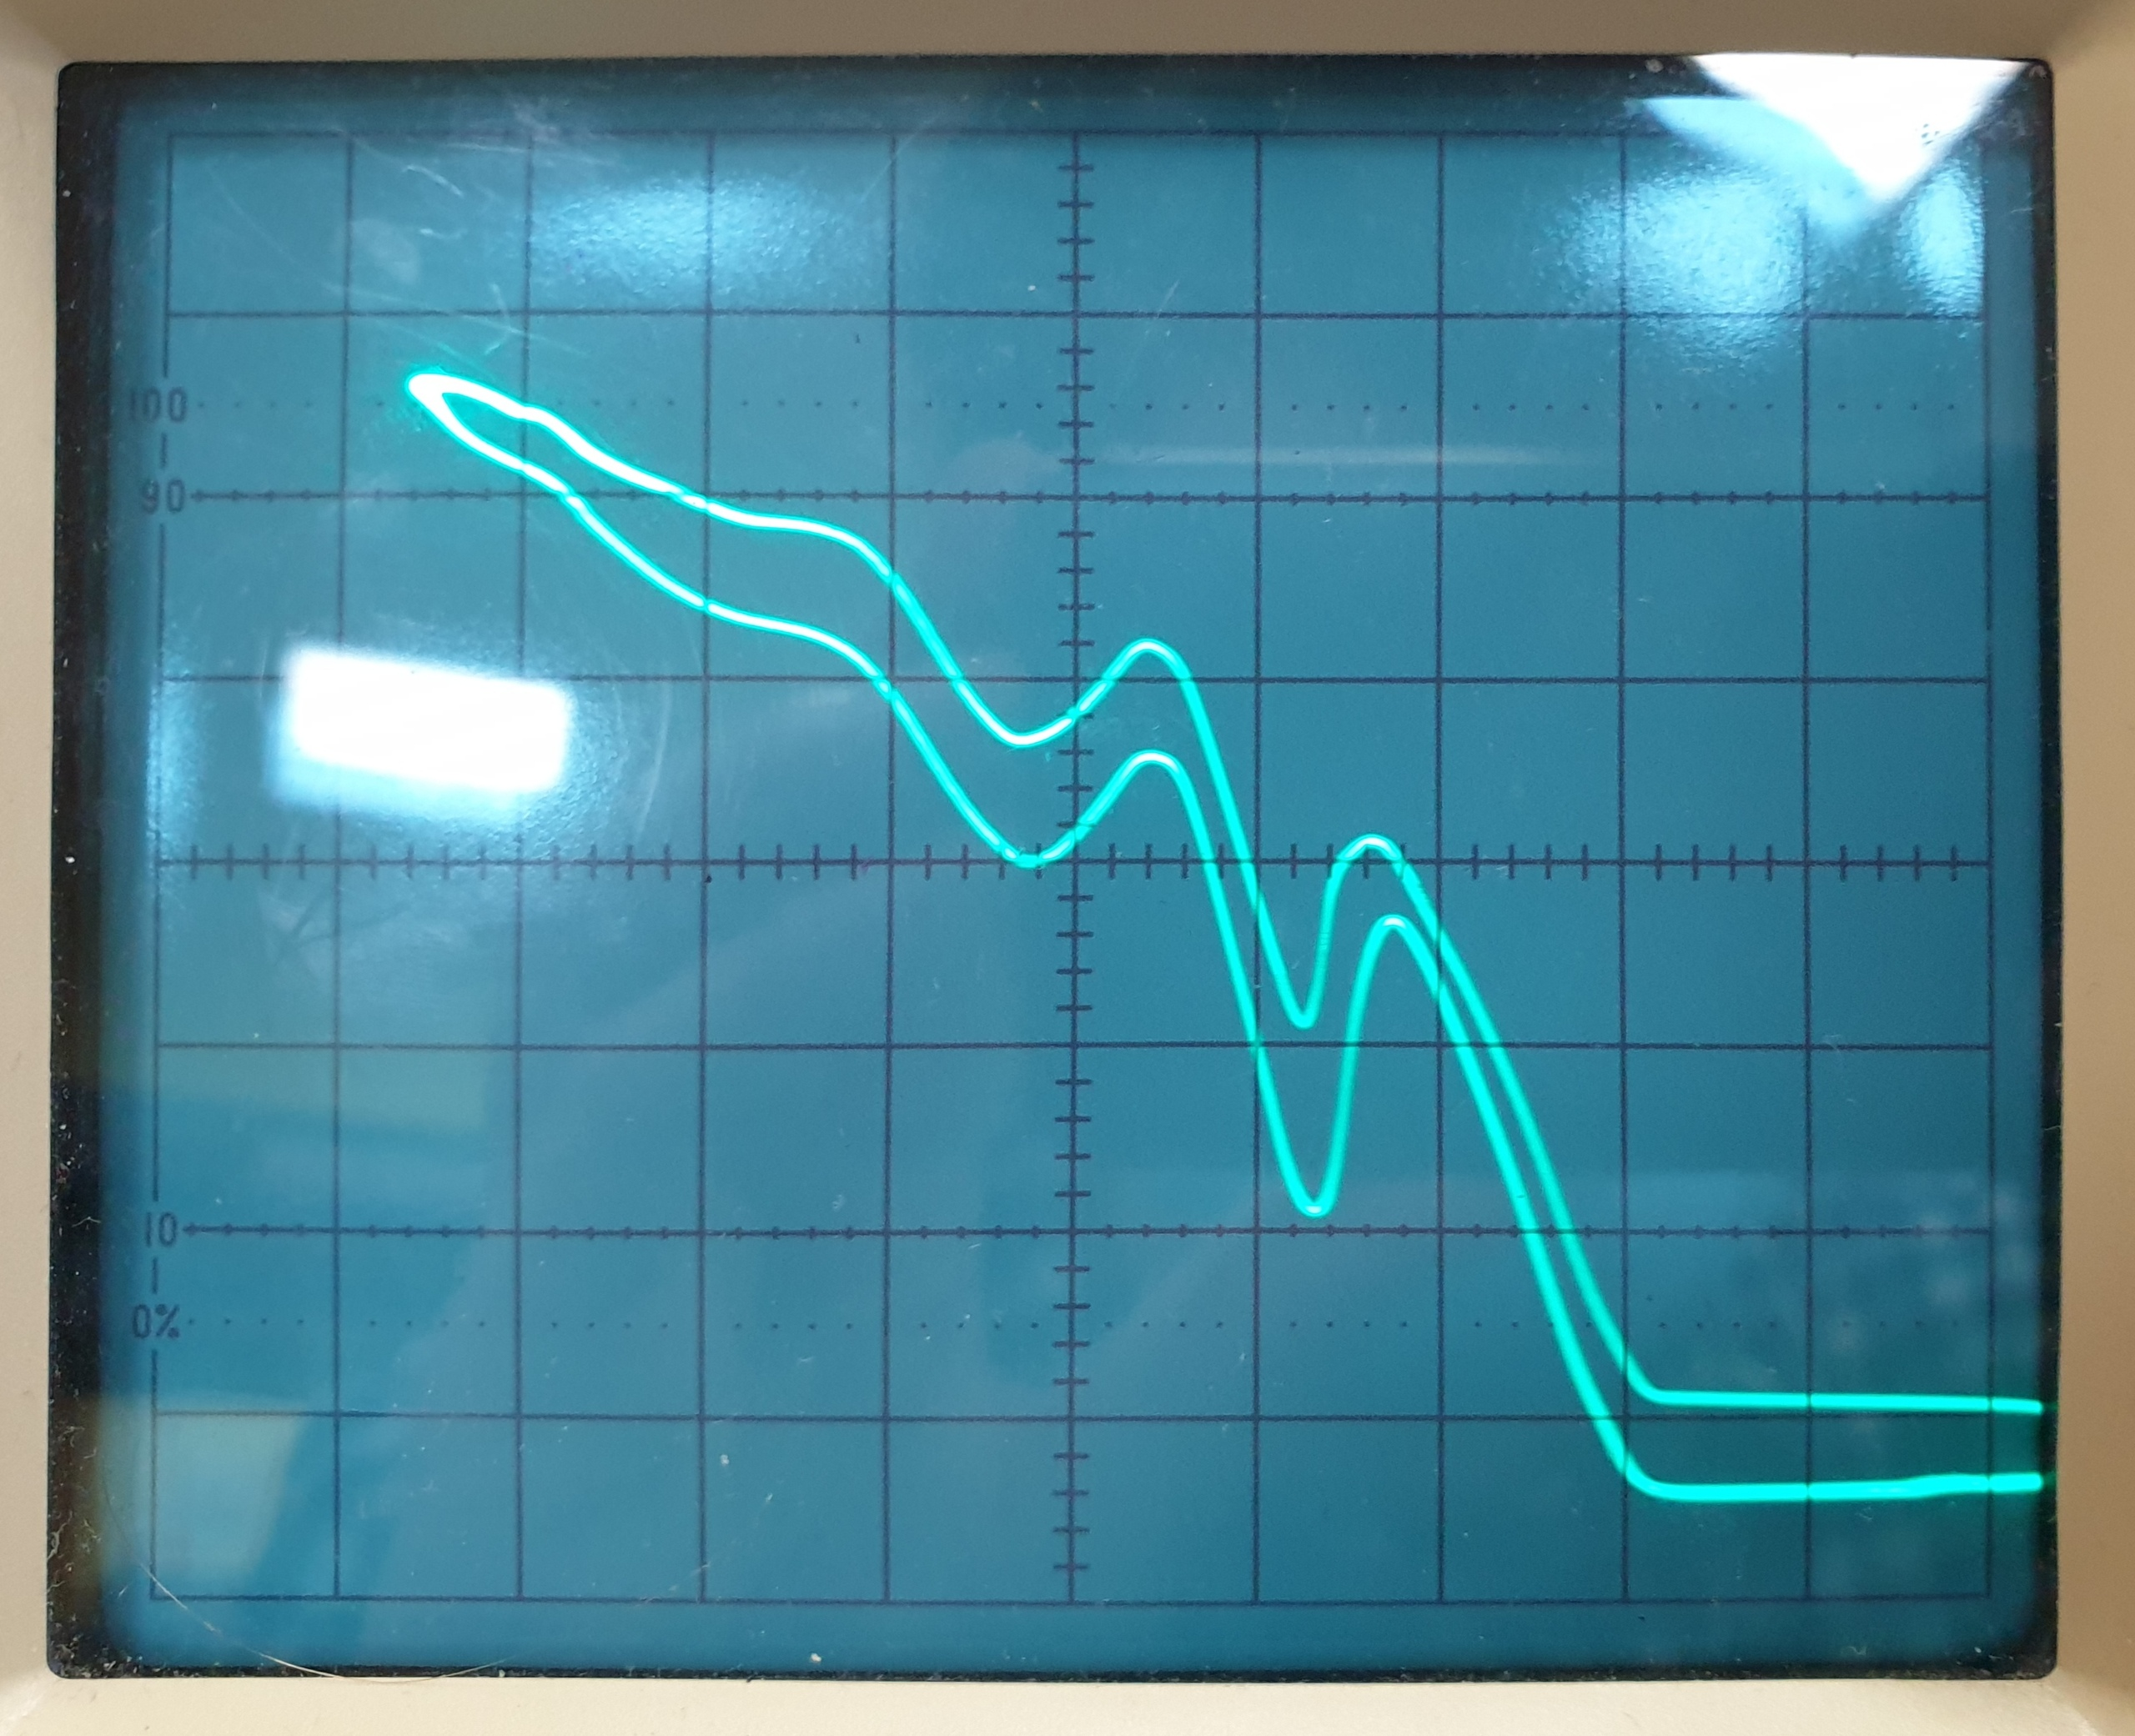
\includegraphics[width=1\linewidth]{din6V} \\ (6B)}
\end{minipage}
\hfill
\begin{minipage}[h]{0.32\linewidth}
\center{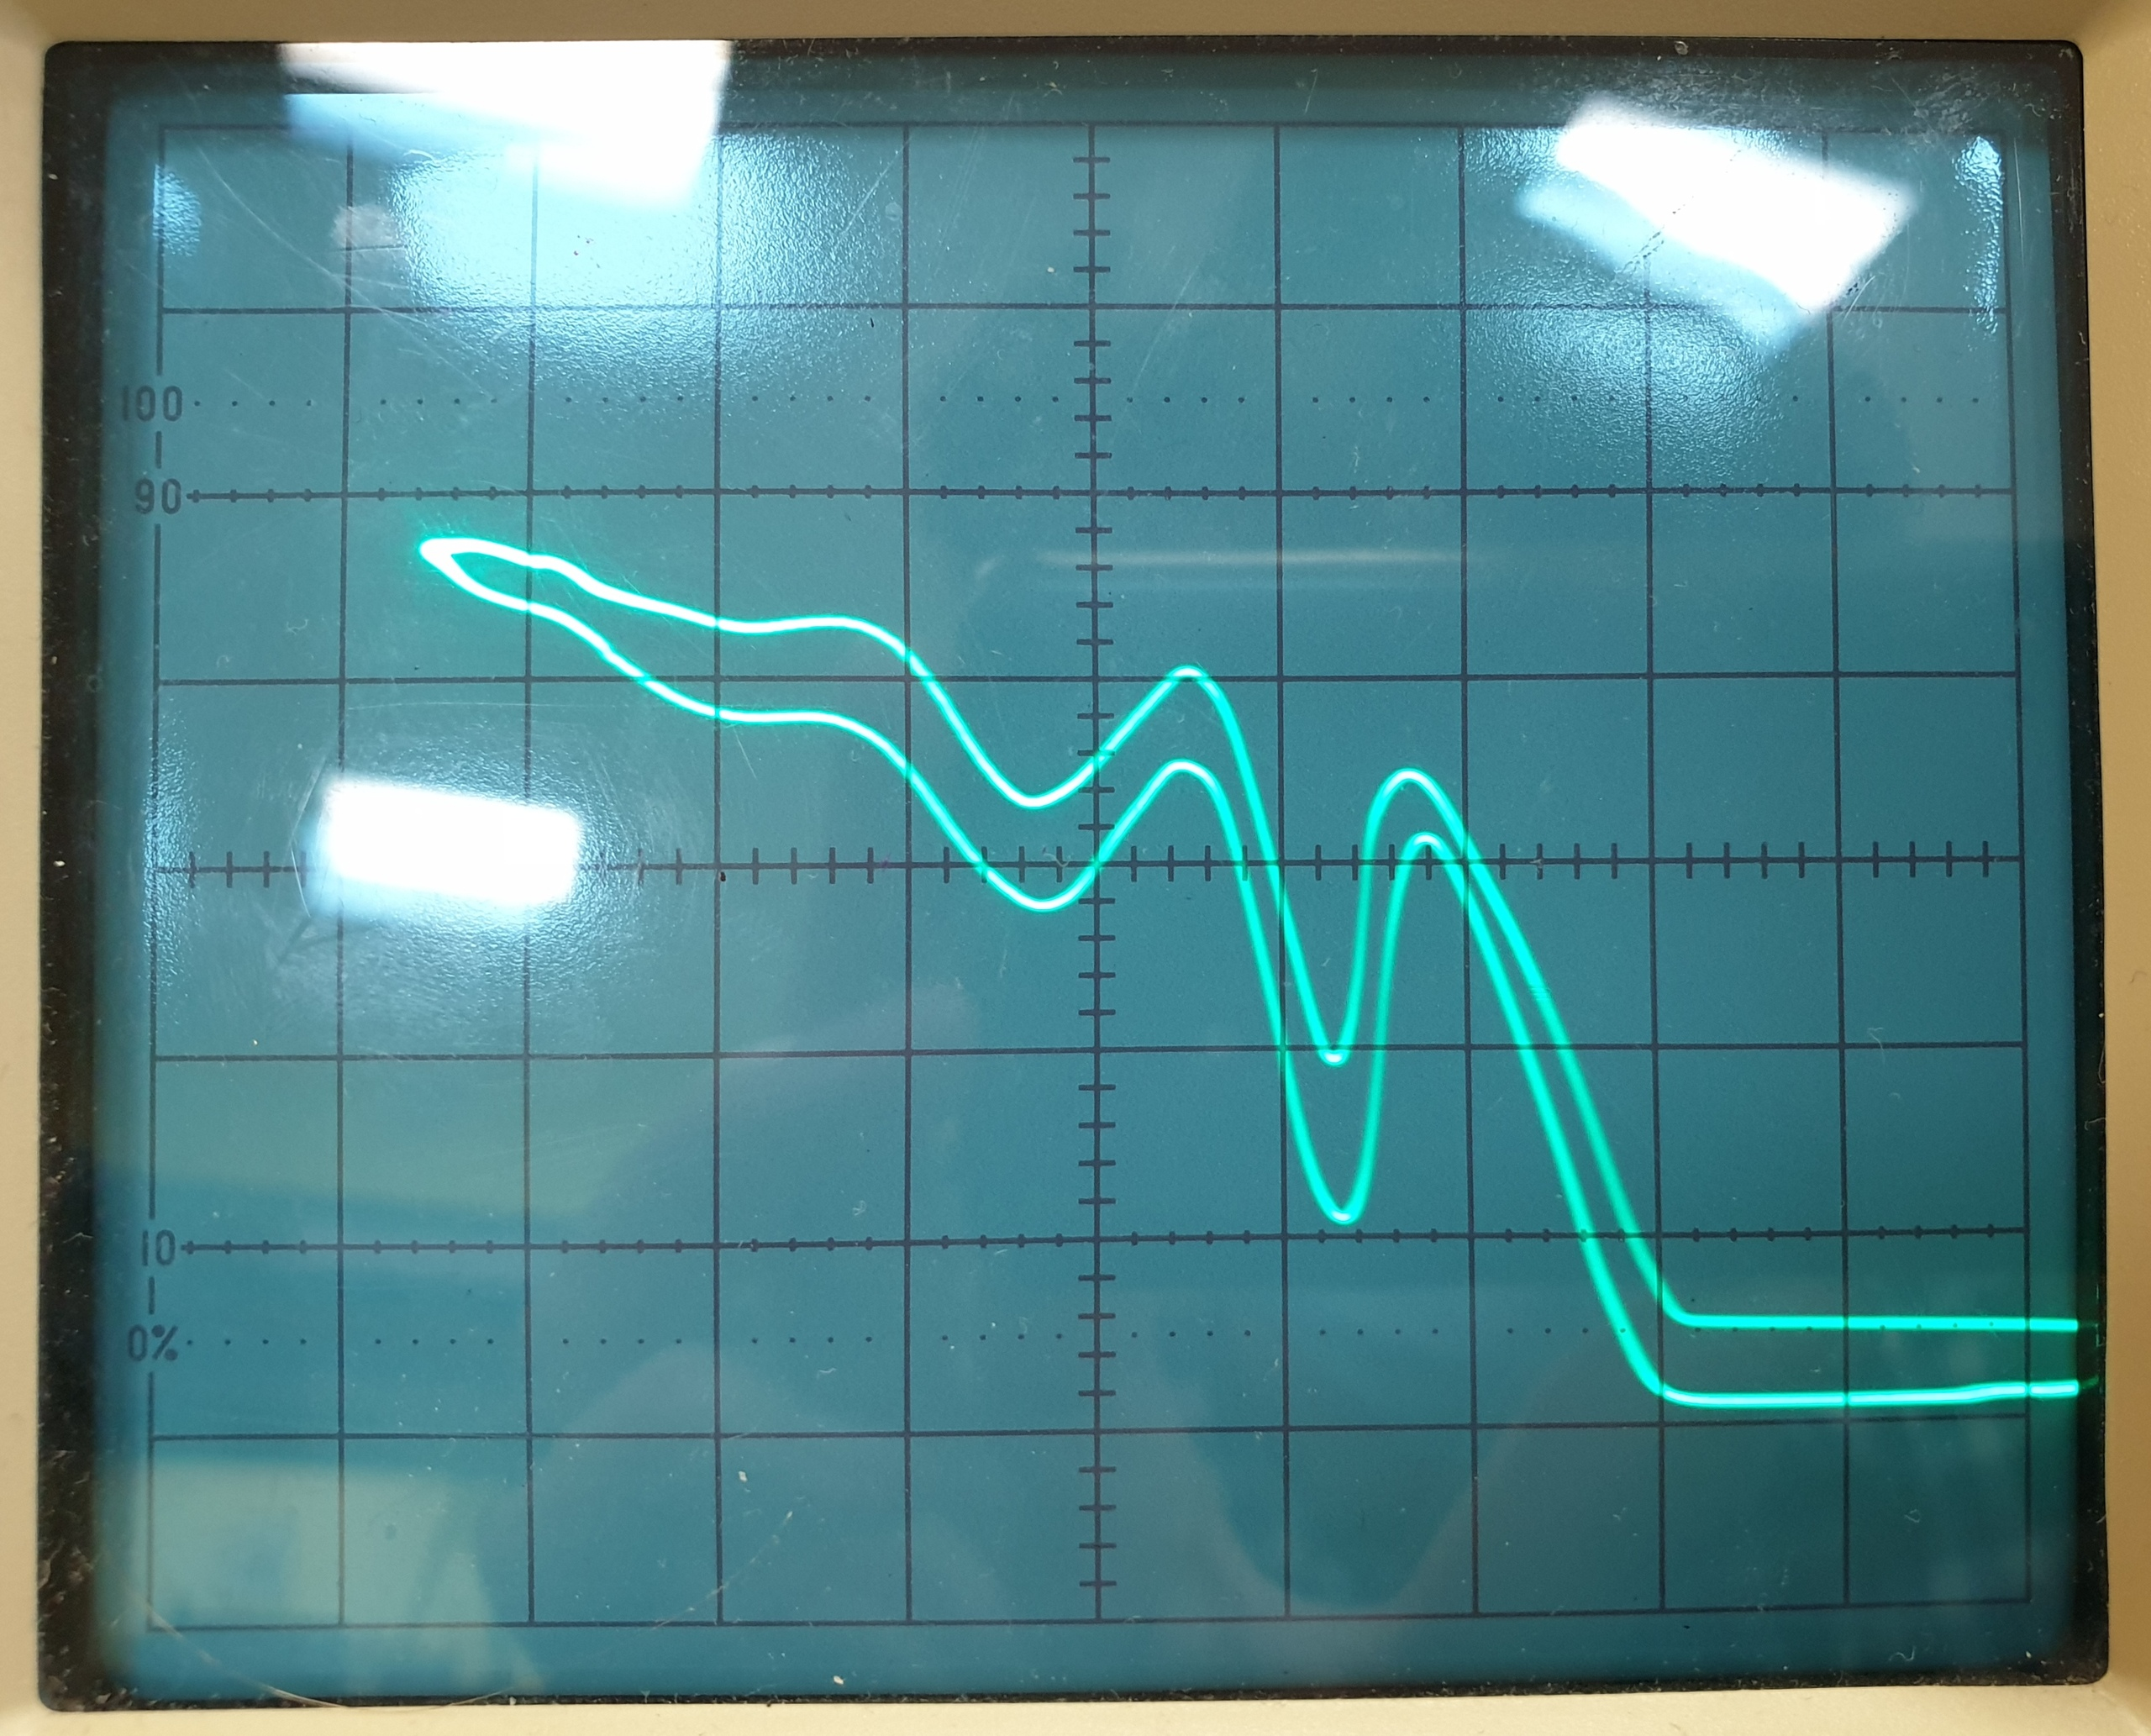
\includegraphics[width=1\linewidth]{din8V} \\ (8B)}
\end{minipage}
\ECaption{Зависимость $I_k(V_a)$. Наличие второй линии связано с гистерезисом и не может быть полностью устранено, однако при этом $\Delta V$ одинаково для прямого/обратного направлений. Для фото кривые были сжаты, однако измерение проводилось на достоверных значениях цены деления осциллографа.}
\end{figure}


Зная масштаб шкалы, находим энергию первого уровня для соответствующего задерживающего напряжения (таблица 1).
\begin{table}[h!]
\begin{center}
\begin{tabular}{|c|c|c|c|}
\hline
\rowcolor[HTML]{9698ED} 
$V_{\text{задерж}}$, B & $\Delta V_{\text{прямой}}$, B & $\Delta V_{\text{обратный}}$, B & $\Delta_{\Delta V}$, B \\ \hline
4                      & 14.5                          & 16                              & 1                      \\ \hline
\rowcolor[HTML]{9698ED} 
6                      & 14.5                          & 15.5                            & 1                      \\ \hline
8                      & 14.5                          & 15.5                            & 1                      \\ \hline
\end{tabular}
\ECaption{Результаты измерения энергии первого уровня атома гелия. Погрешность берется как цена деления. Как видно, значения на прямом и обратном направлении отличаются, но в пределах погрешности.}
\end{center}
\end{table}

Как и ожидалось, от величины задерживающего напряжения зависит лишь четкость картины и количество пиков, а значения энергии (в -Эв) одинаковы. 

Можно сделать промежуточный вывод о том, что измерение обратным ходом будет точнее, так как пики имеют более острую форму, из-за чего легче определить их положения

\section*{Статический метод}

В статическом режиме напряжения и ток измеряются вольтметром и микроамперметром соответственно. Полученные значения представлены на таблице. 
\begin{table}[h]
\begin{center}
\begin{tabular}{|c|c|c|c|c|c|c|c|c|c|}
\hline
\rowcolor[HTML]{6665CD} 
$V = 4$ B     &       &       &       &       &       &       &       &       &       \\ \hline
\rowcolor[HTML]{9698ED} 
$V_a$, B      & 2.17  & 3.52  & 5.22  & 6.29  & 8.14  & 9.64  & 11.22 & 12.89 & 14.53 \\ \hline
$I_k$, $\mu$A & 7     & 10    & 15    & 20    & 25    & 30    & 35    & 40    & 45    \\ \hline
\rowcolor[HTML]{9698ED} 
              & 16.49 & 18.7  & 20.59 & 22.2  & 22.7  & 22.92 & 23.75 & 24.83 & 25.96 \\ \hline
              & 50    & 55    & 57    & 55    & 50    & 45    & 41    & 45    & 50    \\ \hline
\rowcolor[HTML]{9698ED} 
              & 27.37 & 28.59 & 29.74 & 31.02 & 32.31 & 33.68 & 35.1  & 37.18 & 39.37 \\ \hline
              & 55    & 60    & 65    & 70    & 75    & 80    & 85    & 87    & 85    \\ \hline
\rowcolor[HTML]{9698ED} 
              & 40.62 & 43.93 & 48.18 & 51.19 & 52.72 & 55.37 & 57.94 & 69.15 & 77.15 \\ \hline
              & 83    & 81    & 85    & 90    & 92    & 92    & 92    & 92    & 92    \\ \hline
\rowcolor[HTML]{6665CD} 
$V = 8$ B     &       &       &       &       &       &       &       &       &       \\ \hline
\rowcolor[HTML]{9698ED} 
$V_a$, B      & 0.06  & 4.79  & 7.04  & 8.25  & 9.74  & 11.12 & 12.59 & 14.28 & 16    \\ \hline
\rowcolor[HTML]{FFFFFF} 
$I_k$, $\mu$A & 0     & 5     & 10    & 15    & 20    & 25    & 30    & 35    & 40    \\ \hline
\rowcolor[HTML]{9698ED} 
              & 17.68 & 19.64 & 22    & 22.59 & 23.42 & 23.71 & 23.95 & 23.96 & 24.6  \\ \hline
\rowcolor[HTML]{FFFFFF} 
              & 45    & 50    & 51    & 50    & 47    & 45    & 41    & 26    & 20    \\ \hline
\rowcolor[HTML]{9698ED} 
26.03         & 27.4  & 28.37 & 29.35 & 30.25 & 31.27 & 32.49 & 33.66 & 34.8  & 38.19 \\ \hline
\rowcolor[HTML]{FFFFFF} 
18            & 21    & 25    & 30    & 35    & 40    & 45    & 50    & 55    & 60    \\ \hline
\rowcolor[HTML]{9698ED} 
40.64         & 42.06 & 43.67 & 44.72 & 47.23 & 49.45 & 52.26 & 55.32 & 58.64 & 65.08 \\ \hline
\rowcolor[HTML]{FFFFFF} 
57            & 55    & 52    & 50    & 47    & 47    & 50    & 55    & 60    & 63    \\ \hline
\end{tabular}
\ECaption{Результаты измерения зависимостей. В местах, где наблюдаются пики, измерения снимаются с большей точностью. Некоторые точки могут быть измерены недостоверно, так как автор периодически забывал о наличии гистерезиса.}
\end{center}
\end{table}

Построим ВАХ системы на графиках (рис.3).

\begin{figure}[h]
\begin{minipage}[h]{0.5\linewidth}
\center{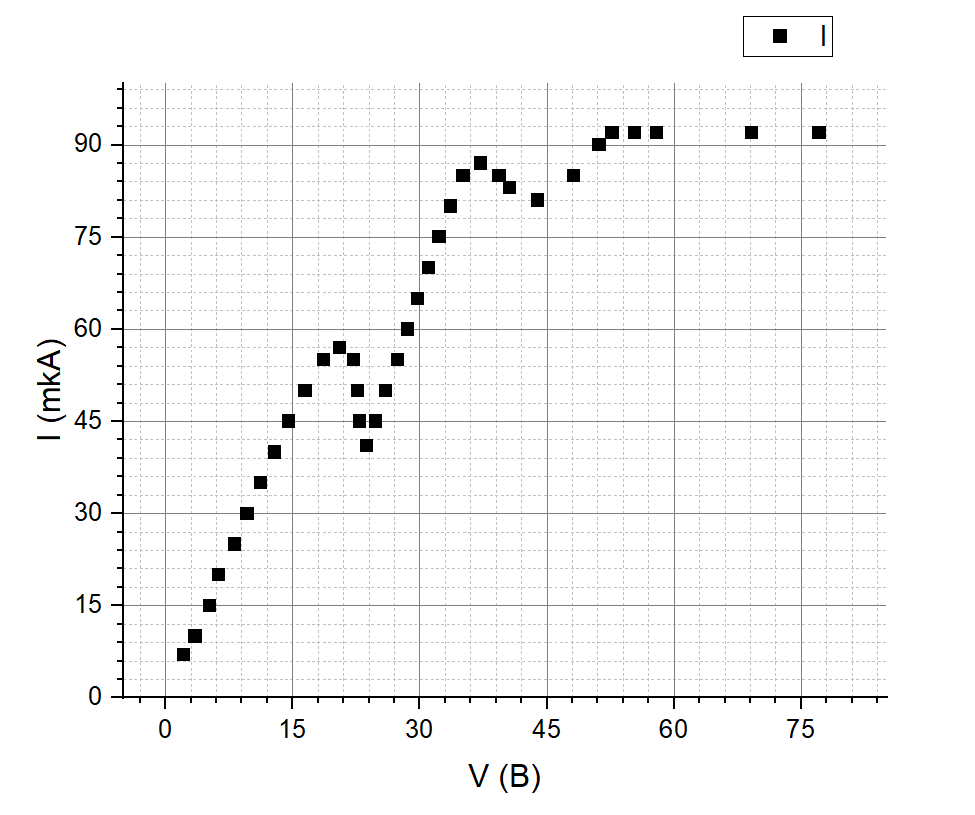
\includegraphics[width=1\linewidth]{gr1} \\ (4B)}
\end{minipage}
\hfill
\begin{minipage}[h]{0.5\linewidth}
\center{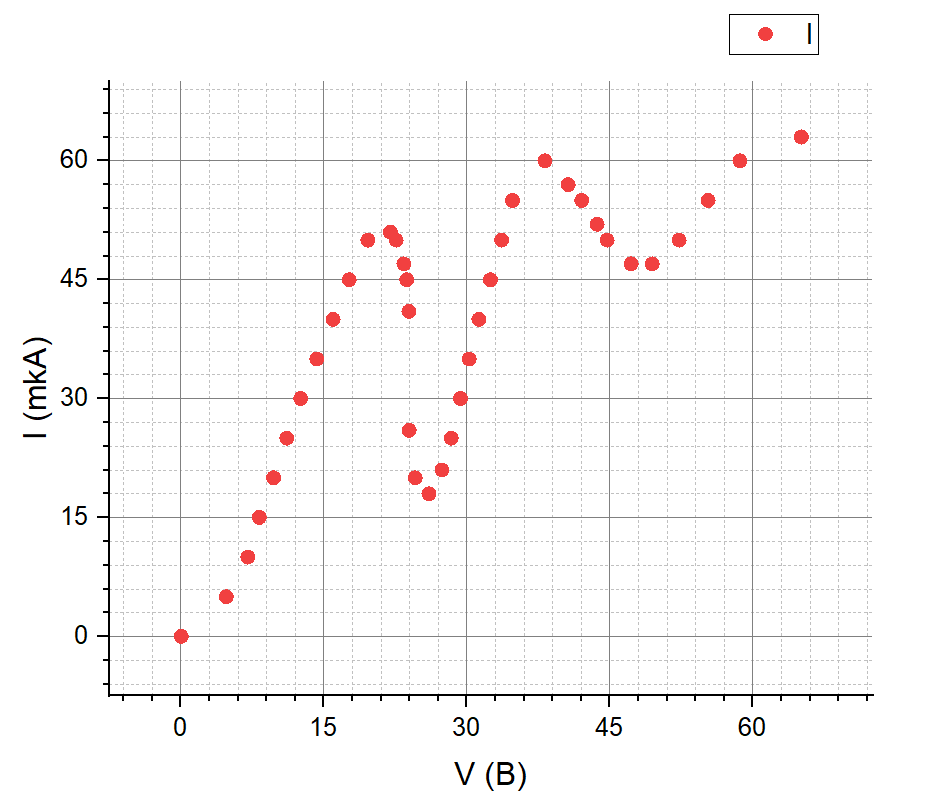
\includegraphics[width=1\linewidth]{gr2} \\ (8B)}
\end{minipage}
\caption{Пики для соответствующих задерживающих напряжений. Картина  подтверждает полученные ранее выводы о влиянии задерживающего напряжения на картину опыта Франка-Герца.}
\label{ris:image1}
\end{figure}

Можно оценить положения пика через вершину пораболы, или пересечение каскадных прямых пика, однако в данном случае такая оценка с учетом погрешности не будет отличаться от пикового значения в данных. Таким образом, оцениваем $\Delta V$ как разность пиковых значений на графике. 
\newpage
Результаты в виде энергии ионизации:
\[E = 16.59 \pm  \text{ эВ, (для 4В)},\] 
\[E = 16.19 \text{ эВ, (для 8В)}. \]

\section*{Вывод}

Данный эксперимент действительно подтверждает дискретную природу уровней энергии в атоме гелия, показывая достаточно четкую картину ВАХ. 

Табличное значение для энергии ионизации первого возбужденного состояния гелия составляет 19.82 эВ, что не совпадает с результатами моего эксперимента. Однако при этом результаты измерения динамическим и статическим методами практически совпадают, что позволяет сделать следующий вывод: либо при обработке результаты были интерпретированны систематически неверно, либо проблемы в установке: в камере присутствует смесь гелия с воздухом, а не чистый газ. Так же влияние гистерезиса было бы заметно на кривой, так что проведение эксперимента не должно было привести к такому результату.

В любом случае, статический метод в таких условиях приводит к большей точности, однако это следствие несовершенства такого осциллографа. Если бы можно было сильнее увеличить задерживающий потенциал, то можно было бы получить динамическим методом более точные результаты.





























































\end{document}